\documentclass[11pt]{article}
\usepackage{multicol}
\setlength{\columnseprule}{1pt} % separation line between columns
\setlength{\parindent}{0pt} % paragraph indentation

\usepackage[top=2cm, bottom=2cm, left=2cm, right=2cm]{geometry}
\usepackage[T1]{fontenc}
\usepackage[francais]{babel}
\usepackage{textcomp}

\usepackage{hyperref}
\hypersetup{
	colorlinks=true,       	% false: boxed links; true: colored links
	linkcolor=black,          	% color of internal links
	urlcolor=blue,           	% color of external links
	citecolor=blue
}

\usepackage{dashrule}
\usepackage{wrapfig}
\usepackage{graphicx}
\usepackage{enumitem}
\usepackage{wrapfig}
\usepackage{cancel} % diagonal strikeout
\usepackage[margin=1cm]{caption}
\setdescription{leftmargin=1cm,labelindent=0.5cm}

\usepackage{amsmath}
\usepackage{amsfonts}
\newcommand\mathd[0]{\mathrm{d}}

\usepackage{blindtext}

% Colors
\usepackage[usenames,dvipsnames]{xcolor}

% Colored frame
\usepackage{framed}
\definecolor{shadecolor}{rgb}{0.96,0.96,0.96}
\definecolor{TFFrameColor}{rgb}{0.96,0.96,0.96}
\definecolor{TFTitleColor}{rgb}{0.00,0.00,0.00}

% Redefine leftbar envvironment
\newlength{\leftbarwidth}
\setlength{\leftbarwidth}{1pt}
\newlength{\leftbarsep}
\setlength{\leftbarsep}{10pt}

\newcommand*{\leftbarcolorcmd}{\color{leftbarcolor}} % as a command to be more flexible
\colorlet{leftbarcolor}{gray}

\renewenvironment{leftbar}{%
    \def\FrameCommand{{\leftbarcolorcmd{\vrule width \leftbarwidth\relax\hspace {\leftbarsep}}}}%
    \MakeFramed {\advance \hsize -\width \FrameRestore }%
}{%
    \endMakeFramed
}

\usepackage{listings}
\definecolor{dkgreen}{rgb}{0,0.6,0}
\definecolor{gray}{rgb}{0.5,0.5,0.5}
\definecolor{mauve}{rgb}{0.58,0,0.82}
\definecolor{blue}{rgb}{0,0,0.7}
\lstset{
	language=Matlab,
	basicstyle=\scriptsize,
	numbers=left,                   % where to put the line-numbers
  	numberstyle=\tiny\color{gray},
	commentstyle=\color{dkgreen},
	frame=single,                   % adds a frame around the code
 	rulecolor=\color{black},
	emph={},
	emphstyle=\color{mauve},
	morekeywords={},
	keywordstyle={\color{blue}},
	showstringspaces=false,
  	tabsize=4
}

% Title page
\title{PR-3001M\\
\small{Systèmes dynamiques}}
\date{\today}

\begin{document}
\maketitle
\newpage

\tableofcontents
\newpage

\section{Modèle physique}
\begin{figure}[h!]
	\centering
	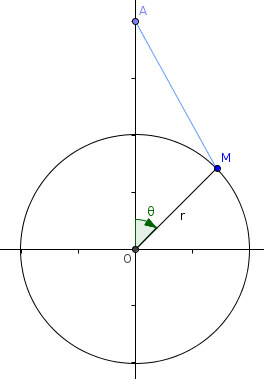
\includegraphics[scale=0.6]{Figures/sch1.png}
\end{figure}

Nous avons utilisé la conservation de l'énergie mécanique pour trouver l'équation différentielle du système.

\subsection{Conservation de l'énergie mécanique}
L'énergie mécanique est la somme de l'énergie cinétique et de l'énergie potentielle. Celle-ci reste constante au cours du temps en l'absence de frottements.

\begin{flalign*}
	Em &= Ep + Ec&\\
	   &= Epp + Epe + Ec,&
\end{flalign*}
avec $Em$ l'énergie mécanique, $Ep$ l'énergie potentielle, $Epp$ l'énergie potentielle de pesanteur, $Epe$ l'énergie potentielle élastique du ressort et $Ec$ l'énergie cinétique.

\paragraph{Énergie cinétique} \mbox{}\\
\begin{flalign*}
	Ec &= \frac{1}{2} m v^2 \text{, avec } v = r \dot{\theta}&\\
	   &= \frac{1}{2} m r^2 \dot{\theta}^2&
\end{flalign*}
\newpage

\paragraph{Énergie potentielle de pesanteur}\mbox{}\\
\begin{figure}[h]
	\centering
	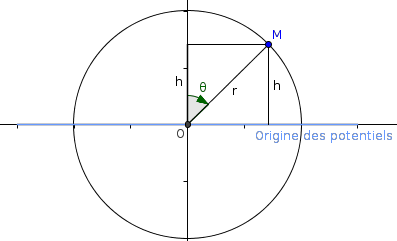
\includegraphics[scale=0.6]{Figures/sch2.png}
\end{figure}

\setlength{\abovedisplayskip}{0pt}
\begin{multicols}{2}
	\begin{align*}
		&\cos(\theta) = \frac{h}{r}&\\
		&h = r \cos(\theta)&
	\end{align*}

	\begin{align*}
    	Epp &= mgh&\\
	        &= mgrcos(\theta)&
	\end{align*}
\end{multicols}
\setlength{\abovedisplayskip}{8pt}


\paragraph{Énergie potentielle élastique du ressort}
\begin{flalign*}
	&Epe = \frac{1}{2}k(l -l_0)&
\end{flalign*}
avec $l_0$: longueur du ressort au repos, $l$: longueur du ressort et $k$: constante de raideur du ressort.\\

\begin{multicols}{2}
\begingroup
	\centering
	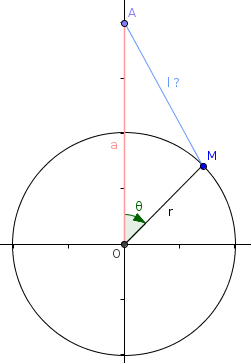
\includegraphics[scale=0.6]{Figures/sch3.png}
\endgroup

\underline{Théorème d'Al-Kashi}:
\begin{leftbar}
$\alpha$, $\beta$, $\gamma$ angles\\
a, b, c côtés opposés aux angles\\
$c^2 = a^2 + b^2 - 2ab\cos\gamma$
\end{leftbar}

Dans notre cas (voir figure ci-contre) :
\begin{flalign*}
l^2 &= a^2 + r^2 - 2ar\cos\theta&\\
l &= \sqrt{a^2 + r^2 - 2ar\cos\theta}&\\
Epe &= \frac{1}{2} k (\sqrt{a^2 + r^2 - 2ar\cos\theta} - l_0)^2&
\end{flalign*}
\end{multicols}

\paragraph{Intégrale première de la conservation de l'énergie}
\begin{flalign*}
	Em &= Epp + Epe + Ec&\\
	   &= \frac{1}{2}mr^2 \dot{\theta}^2
	      + mgr\cos\theta
	      + \frac{1}{2}k \left(\sqrt{a^2 + r^2 - 2ar\cos\theta} - l_0\right)^2&
\end{flalign*}

\underline{On divise par $mr^2$} :
\begin{flalign*}
\frac{Em}{mr^2} &= \frac{1}{2} \dot{\theta}^2
                   + \frac{g}{r}\cos\theta
                   + \frac{1}{2} \frac{k}{mr^2}
                     \left(
                   		\sqrt{a^2 + r^2 - 2ar\cos\theta} - l_0
                   	 \right)^2&\\
\end{flalign*}

\underline{Par hypothèse, $g=r=l_0$ et $\frac{k}{m}=\frac{\lambda}{\mu}$} :
\begin{flalign*}
	\frac{Em}{mr^2} &= \frac{1}{2} \dot{\theta}^2
	                   + \cos\theta
	                   + \frac{1}{2}\frac{k}{mr^2}
	                    \left(
	                   		r\sqrt{\frac{a^2}{r^2} + 1 - 2\frac{a}{r}\cos\theta} - r
	                   	\right)^2&\\
	&= \frac{1}{2} \dot{\theta}^2
	   + \cos\theta
	   + \frac{1}{2} \frac{k}{m}
	     \left(
	   		\sqrt{\frac{a^2}{r^2} + 1 - 2\frac{a}{r}\cos\theta} - 1
	   	\right)^2&
\end{flalign*}

\begin{flalign*}
	&\boxed{
		\frac{Em}{mr^2} = \frac{1}{2} \dot{\theta}^2
		                  + \cos\theta
		                  + \frac{1}{2} \frac{\lambda}{\mu}
		                    \left(
		                  		\sqrt{\mu^2 + 1 - 2\mu\cos\theta} - 1
		                  	\right)^2
	}&
\end{flalign*}

$\displaystyle C = \frac{1}{2} \dot{\theta}^2 + H(\theta)$ avec
$\begin{cases}
	C = \frac{Em}{mr^2}\\
	H(\theta) = \cos(\theta) + \frac{1}{2} \frac{\lambda}{\mu} (\sqrt{\mu^2 + 1 - 2\mu\cos(\theta)} - 1)^2
\end{cases}$

\paragraph{Équation différentielle}\mbox{}\\
Pour trouver l'équation différentielle, il faut dériver l'intégrale première trouvée précédemment.

\begin{flalign*}
	C &= \frac{1}{2}\dot{\theta}^2 + H(\theta)&\\
	0 &= \frac{1}{2} \frac{\mathd}{\mathd t}\dot{\theta}^2 + \frac{\mathd}{\mathd t}H(\theta)&\\
	&= \ddot{\theta}\dot{\theta} + \dot{\theta} \frac{\mathd}{\mathd \theta}H(\theta), \quad \dot{\theta} \neq 0&\\
	&= \ddot{\theta} + \frac{\mathd}{\mathd \theta}H(\theta)&\\
	&= \ddot{\theta} + \frac{\mathd}{\mathd \theta}\left( \cos(\theta) + \frac{1}{2} \frac{\lambda}{\mu} (\sqrt{\mu^2 + 1 - 2\mu\cos\theta} - 1)^2 \right)&\\
	&= \ddot{\theta} -\sin\theta + \frac{1}{2}\frac{\lambda}{\mu}\frac{\mathd}{\mathd \theta}\left( (\sqrt{\mu^2 + 1 - 2\mu\cos\theta} - 1)^2 \right)&\\
	&= \ddot{\theta} -\sin\theta + \frac{1}{2}\frac{\lambda}{\mu}\frac{\mathd}{\mathd \theta}\left( f(\theta)^2 \right)&\\
	&= \ddot{\theta} -\sin\theta + \frac{\lambda}{\mu}f'(\theta)f(\theta)&\\
	&= \ddot{\theta} - \sin\theta + \frac{\lambda}{\mu} \left(
		\mu \sin(\theta) - \frac{\mu \sin\theta}{\sqrt{\mu^2 +1 -2\mu \cos\theta}}
	\right)&
\end{flalign*}

\begin{flalign*}
	&\boxed{
		0 = \ddot{\theta}
		    + \sin\theta
		      \left(
		      	-1 +\lambda
		    	- \frac{\lambda}{\sqrt{\mu^2 +1 -2\mu \cos\theta}}
		      \right)
	}&
\end{flalign*}

$\displaystyle  \ddot{\theta} + h(\mu,\lambda ; \theta) = 0$ avec
$\begin{cases}
	h(\mu,\lambda ; \theta) = \sin\theta\left(-1 +\lambda -\frac{\lambda}{\sqrt{\mu^2 +1 -2\mu \cos\theta}} \right)\\
	\lambda > 0\\
	\mu > 0
\end{cases}$

\newpage
\section{Cas sans frottement}
\subsection{Points d'équilibre}
Soit $\displaystyle h(\theta) = \sin\theta\left(-1 +\lambda -\frac{\lambda}{\sqrt{\mu^2 +1 -2\mu \cos\theta}} \right)$, si $h(\theta^*) = 0$, alors le point $\theta^*$ est un point d'équilibre du système. Un point d'équilibre vérifie donc une de ces deux équations:

\begin{flalign*}
	&\begin{cases}
		\sin\theta^* = 0\\
		-1 +\lambda -\dfrac{\lambda}{\sqrt{\mu^2 +1 -2\mu \cos\theta^*}} = 0
	\end{cases}&
\end{flalign*}

\paragraph{Premier cas}
\begin{flalign*}
	\sin\theta^* &= 0&\\
	\theta^* &= k\pi, \text{ avec } k\in\mathbb{Z} &
\end{flalign*}
Le système possède donc au moins deux points d'équilibre (qui se répètent de manière périodique), $\theta^* = 0$ et $\theta^* = \pi$.

\paragraph{Second cas}
\begin{multicols}{2}
	\begin{flalign*}
		-1 +\lambda -\frac{\lambda}{\sqrt{\mu^2 +1 -2\mu \cos\theta^*}} &= 0&\\
		\frac{1}{\sqrt{\mu^2 +1 -2\mu \cos\theta^*}} &= \frac{\lambda - 1}{\lambda}&\\
		\mu^2 +1 -2\mu \cos\theta^* &= \left(\frac{\lambda}{\lambda - 1}\right)^2&
	\end{flalign*}
	\begin{flalign*}
		&\cos\theta^* = -\left(\left(\frac{\lambda}{\lambda - 1}\right)^2 -\mu^2 -1\right)\frac{1}{2\mu}&\\
	\end{flalign*}
	\vfill
	\columnbreak

	\hfill\\\\
	\begin{flalign*}
	\mu^2 +1 -2\mu\cos{\theta^*} > 0 \Rightarrow& \frac{\lambda}{\lambda - 1} > 0&\\
		                                        & \lambda > 1&
	\end{flalign*}
\end{multicols}
Dans le cas où cette équation admet des solutions, le système aura deux points d'équilibre supplémentaires ($\cos(\theta) = \cos(-\theta)$ ).\\

Recherche des condtitions d'existence des deux points d'équilibres supplémentaires pour\\ $\cos\theta^* = -\left(\left(\frac{\lambda}{\lambda - 1}\right)^2 -\mu^2 -1\right)\frac{1}{2\mu}$.

\begin{flalign*}
	&\begin{cases}
		-\left(\left(\frac{\lambda}{\lambda - 1}\right)^2 -\mu^2 -1\right)\frac{1}{2\mu} > -1& (1)\\
		-\left(\left(\frac{\lambda}{\lambda - 1}\right)^2 -\mu^2 -1\right)\frac{1}{2\mu} < 1& (2)
	\end{cases}&
\end{flalign*}

\underline{Résolution de (1)}:
\begin{flalign*}
	-\left(\left(\frac{\lambda}{\lambda - 1}\right)^2 -\mu^2 -1\right)\frac{1}{2\mu} &> -1&\\
	\left(\frac{\lambda}{\lambda - 1}\right)^2 -\mu^2 -1 &< 2\mu&\\
	\left(\frac{\lambda}{\lambda - 1}\right)^2 -\mu^2 -1 - 2\mu &< 0&\\
	\left(\frac{\lambda}{\lambda - 1}\right)^2 - (\mu + 1)^2 &< 0&\\
	\left(\frac{\lambda}{\lambda - 1} -\mu -1\right)\left(\frac{\lambda}{\lambda - 1} +\mu +1\right) &< 0&\\
\end{flalign*}

$\Rightarrow \mu > \frac{\lambda}{\lambda -1} - 1$ ou $\mu > -\frac{\lambda}{\lambda -1} - 1$\\

\underline{Résolution de (2)}:
\begin{flalign*}
	-\left(\left(\frac{\lambda}{\lambda - 1}\right)^2 -\mu^2 -1\right)\frac{1}{2\mu} &< 1&\\
	\left(\frac{\lambda}{\lambda - 1}\right)^2 -\mu^2 -1 &> -2\mu&\\
	%
	\left(\frac{\lambda}{\lambda - 1}\right)^2 - (\mu - 1)^2 &> 0&\\
	\left(\frac{\lambda}{\lambda - 1} -\mu +1\right)\left(\frac{\lambda}{\lambda - 1} +\mu -1\right) &> 0&\\
\end{flalign*}

$\Rightarrow \mu < \frac{\lambda}{\lambda -1} + 1$ ou $\mu < -\frac{\lambda}{\lambda -1} + 1$\\

\underline{(1) et (2)}:\\

$\mu > 0$ et $\lambda > 1$, donc seules les solutions $\mu>\frac{\lambda}{\lambda - 1} - 1$ et $\mu<\frac{\lambda}{\lambda - 1} + 1$ sont possibles.\\
$\rightarrow \boxed{\displaystyle \mu \in \left] \frac{\lambda}{\lambda - 1}-1 ; \frac{\lambda}{\lambda - 1}+1 \right[}$\\

Application numérique pour $\lambda = 2$ : $\mu \in ]1;3[$.

\paragraph{Conclusion} \mbox{}\\
Le système possède au moins deux points d'équilibre: $\theta^* = 0$ et $\theta^* = \pi$, et au plus 4 points d'équilibre si $\displaystyle \mu \in \left] \frac{\lambda}{\lambda - 1}-1 ; \frac{\lambda}{\lambda - 1}+1 \right[$. Ces points d'équilibre peuvent être stables ou instables, et il y a alternance entre stabilité et instabilité.

\newpage
\paragraph{Construction du tableau dans Matlab} \mbox{}\\
\begin{figure}[h!]
	\centering
	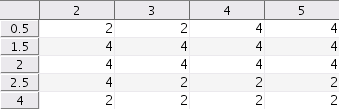
\includegraphics[scale=0.65]{Figures/rapport_nbequi.png}
	\caption{Nombre de points d'équilibre en fonction de $\lambda$ (colonnes) et $\mu$ (lignes)}
\end{figure}

\begin{lstlisting}
function pr3001_B
	lambda_vector=[1 2 3 4 5];
	mu=[0.5 1.5 2 2.5 4];
	...
	displayNbEqui(lambda_vector, mu);
	...
end

% Affiche le nombre de points d'équilibre en fonction de lambda et mu dans
% un tableau.
function displayNbEqui(lambda, mu)
    Z = nbEqui(lambda, mu);

    f = figure('name', 'Nombre de points d''équilibre(lambda, mu)', 'Position', [0 0 600 350]);
    t = uitable('Parent', f, 'Position', [50 700 500 150]);
    set(t, 'Data', Z, 'ColumnName', lambda, 'RowName', mu)
end

% Calcule le nombre de points d'équilibre pour chaque lambda et mu
% (vecteurs). Retourne une matrice (ligne: taille de lambda, colonne: taille de
% mu).
function z=nbEqui(lambda, mu)
    z = zeros(length(mu), length(lambda));

    for i=1:length(mu)
        for j=1:length(lambda)
            if (mu(i) < (lambda(j)/(lambda(j)-1)) + 1) && (mu(i) > (lambda(j)/(lambda(j)-1)) - 1)
                z(i,j) = 4;
            else
                z(i,j) = 2;
            end
        end
    end
end
\end{lstlisting}
La fonction \emph{nbEqui} vérifie la condition $\displaystyle \mu \in \left] \frac{\lambda}{\lambda - 1}-1 ; \frac{\lambda}{\lambda - 1}+1 \right[$ et remplit un tableau à 2 dimensions en fonction de $\lambda$ et $\mu$. A chaque couple de $\lambda$ et $\mu$ est associé un nombre de points d'équilibre. La fonction \emph{displayNbEqui} affiche ensuite le tableau dans l'UI.

\newpage
\subsection{Portrait de phase}
\begin{figure}[h!]
	\centering
	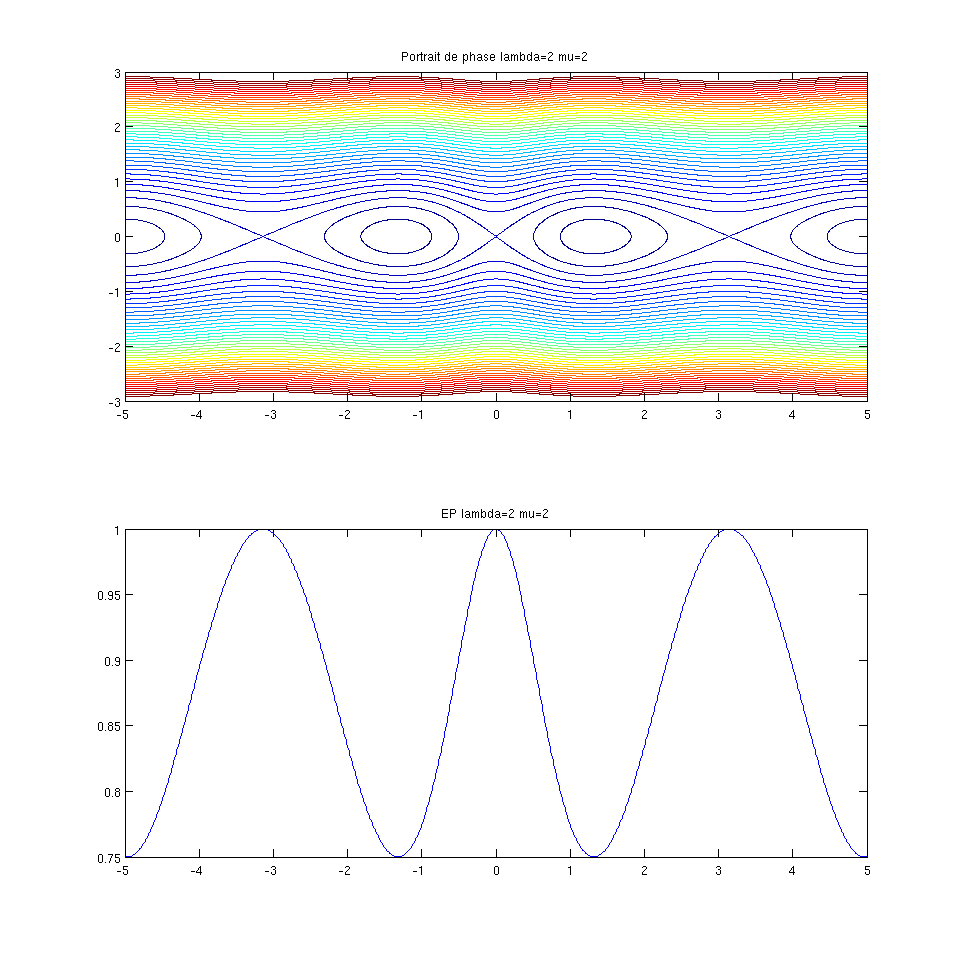
\includegraphics[scale=0.55]{Figures/rapport_figportraitphasemu2.png}
	\caption{Portrait de phase (haut) et énergie potentielle (bas) pour $\lambda=2$ et $\mu=2$}
	\label{fig:pp_ep_mu2}
\end{figure}

Le portrait de phase représente différentes trajectoires possibles pour le système dans le plan de phase $(\theta,\dot{\theta})$. A chaque couple de conditions initiales $(\theta_0, \omega_0)$ est associé une trajectoire différente.\\

Les trajectoires fermées représentent des mouvements oscillatoires (figure \ref{fig:pp_ep_mu2}, trajectoire de type 1) et les trajectoires ouvertes correspondent à des mouvements révolutifs (figure \ref{fig:pp_ep_mu2}, trajectoire de type 2). Une trajectoire dite séparatrice délimite les mouvements révolutifs des mouvements oscillatoires (figure \ref{fig:pp_ep_mu2}, trajectoire de type 3).\\

On fixe $\lambda = 2$ et on trace le portrait de phase pour différents $\mu$ : 0.5, 1.5, 2, 2.5 et 4. Les portraits de phases sont visibles en annexe (Annexe A).
\begin{leftbar}
\textbf{N.B.} Le cas $\mu=1$ n'est pas traité, $\mu = \frac{a}{r}$ donc $a = r$, et pour $\theta = 0$, le ressort devient ponctuel ce qui n'est physiquement pas possible.
\end{leftbar}

Le portrait de phase ci-dessus (figure \ref{fig:pp_ep_mu2}) correspond au cas $\lambda=2$ et $\mu=2$. On peut observer 4 points d'équilibre alternativement stables (minima de l'EP, entourés par des trajectoires fermées) et instables (maxima locales de l'EP, points selle) aux positions suivantes : 0 (instable), $\cos^{-1}{(1/4)}$ (stable), pi (instable) et $-\cos^{-1}{(1/4)}$ (stable).\\

Enfin, l'observation des portraits de phase confirme la théorie selon laquelle il n'y a que deux points d'équilibre dans certaines conditions (cf. portraits de phase pour $\mu = 0.5$ et $\mu = 4$, avec $\lambda=2$).

\paragraph{Matlab} \mbox{}
\begin{leftbar}
Obtention des positions des points d'équilibre autres que $\theta^* = 0$ et $\theta^* = \pi$ à l'aide de Matlab:
\begin{flalign*}
	&-1 + \lambda - \frac{\lambda}{\sqrt{\mu^2 +1 -2\mu\cos{\theta}}} = 0&
\end{flalign*}
Pour $\lambda=2$ et $\mu = 2$
\begin{lstlisting}[numbers=none]
>> x = solve('-1 + 2 - (2/sqrt(2^2 +1 -2*2*cos(x)))', 'x')
ans =
  acos(1/4)
 -acos(1/4)
\end{lstlisting}
\end{leftbar}

\begin{lstlisting}
function pr3001_B
    % Parametres
    lambda=2;
    mu=[0.5 1.5 2 2.5 4];
    ...
    for i=1:length(mu)
        figure

        % portrait de phase
        subplot(2,1,1)
        portraitPhase(lambda, mu(i));
		...
    end
    ...
end

function portraitPhase(lambda, mu)
    [X,Y]=meshgrid(-5:0.01:5, -3:0.01:3);
    Z=integPrem(lambda, mu, X, Y);
    contour(X, Y, Z, -5:0.1:5)
    title(['Portrait de phase lambda=', num2str(lambda), ' mu=', num2str(mu)]);
end

% Intégrale première
function z=integPrem(lambda, mu, x, y)
    z=0.5*y.^2 + H_IntegPrem(lambda, mu, x);
end
\end{lstlisting}
\newpage

\subsection{Vitesse initiale maximale pour une trajectoire périodique}
Nous souhaitons obtenir la vitesse initiale maximale pour une trajectoire périodique sachant que la position $x_0$ a été fixée à $\frac{\pi}{2}$. La séparatrice, déjà décrite auparavant, est la limite entre les trajectoires décrivant un mouvement oscillatoire et les trajectoires décrivant un mouvement révolutif. Celle-ci relie les points d'équilibre instables, et représente à la fois un mouvement de révolution et un mouvement périodique.
Nous cherchons donc l'intersection entre la trajectoire séparatrice et $\frac{\pi}{2}$. La trajectoire séparatrice qui nous intéresse passe par un des 2 points d'équilibre suivants (voir les deux) : $0$ et $\pi$.\\

\underline{Relations utilisées :}
\begin{flalign*}
	C &= \frac{1}{2} \dot{\theta}^2 + H(\theta)&\\
	\dot{\theta} &= \sqrt{2(C - H(\theta))}
\end{flalign*}

\underline{$\lambda = 2$, $\theta_0=\frac{\pi}{2}$}:
\begin{flalign*}
	\dot{\theta} &= \sqrt{2\left( C - \frac{1}{\mu}\left( \sqrt(\mu^2 + 1) - 1 \right)^2 \right)}&
\end{flalign*}

\underline{Aux points d'équilibre $\theta^*=0$ et $\theta^* = \pi$} :\\
L'énergie mécanique est égale à l'énergie potentielle, en effet la vitesse est nulle aux points d'équilibres, l'énergie cinétique y est donc nulle. Cela nous donne donc $C = H(\theta^*)$.
\begin{flalign*}
	C = H(\theta^*) &= \frac{1}{\mu}\left( \sqrt{\mu^2 +1 -2\mu\cos\theta^*} -1 \right)^2 + cos \theta^*&\\
	H(0) &= \frac{1}{\mu}\left( \sqrt(\mu^2 + 1 -2\mu) - 1 \right)^2 + 1&\\
	H(\pi) &= \frac{1}{\mu}\left( \sqrt(\mu^2 + 1 +2\mu) - 1 \right)^2 - 1&
\end{flalign*}

\begin{leftbar}
	\textbf{N.B.} $H(0) \neq H(\pi)$ sauf pour $\mu=2$ (comme vu à la figure \ref{fig:pp_ep_mu2}) :
	\begin{flalign*}
		\frac{1}{\mu}\left( \sqrt(\mu^2 + 1 -2\mu) - 1 \right)^2 + 1 &= \frac{1}{\mu}\left( \sqrt(\mu^2 + 1 +2\mu) - 1 \right)^2 - 1&\\
		\frac{\mu^2 -\mu -2\sqrt{\mu^2 + 1 -2\mu} +2}{\mu} &= \frac{\mu^2 + \mu -2\sqrt{\mu^2 + 1 + 2\mu} + 2}{\mu}&\\
		-\mu -2\sqrt{(-1 + \mu)^2} &= \mu -2\sqrt{(1 + \mu)^2}&\\
		\mu &= 2 \quad\quad (\mu = \pm 2 \text{, mais } \mu>0)&
	\end{flalign*}
	Pour $\mu=2$, la séparatrice passe par les deux points d'équilibre $\theta^*=0$ et $\theta^*=\pi$.
\end{leftbar}

\paragraph{Matlab}\mbox{}\\
On s'intéresse à la trajectoire qui passe par le point d'équilibre ($\theta^*=0$ ou $\theta^*=\pi$) dont l'énergie potentielle est la plus élevée. En effet la séparatrice passe par des points d'équilibres instables, c'est-à-dire les points dont l'énergie est la plus élevée.

\begin{leftbar}
\textbf{Exemple :} $\mu = 4$
\begin{flalign*}
	H(0) &= \frac{1}{4}\left( \sqrt{4^2 + 1 -2*4} - 1 \right)^2 + 1 = 2&\\
	H(\pi) &= \frac{1}{4}\left( \sqrt{4^2 + 1 +2*4} - 1 \right)^2 - 1 = 3&\\
	H(\pi) &> H(0)&
\end{flalign*}
\begin{flalign*}
	C &= H(\pi) = 3 \text{, de plus}\\
	C &= \frac{1}{2}\dot{\theta}^2 + \frac{1}{\mu}\left( \sqrt{\mu^2 + 1} -1 \right)^2&\\
	\omega_{0max} &= \sqrt{2\left( \left( C - \frac{1}{\mu}\left( \sqrt{\mu^2 + 1} - 1 \right) \right)^2\right)} = 1.0598&
\end{flalign*}
\end{leftbar}

\begin{figure}[h!]
	\centering
	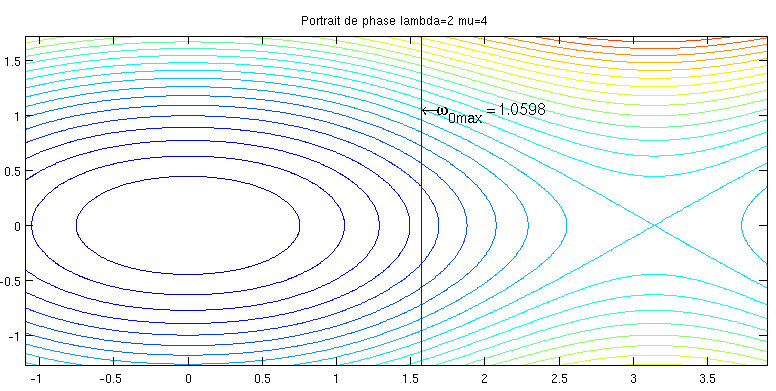
\includegraphics[scale=0.65]{Figures/rapport_figomega0.png}
	\caption{$\omega_{0max}$ sur le portrait de phase pour $\lambda = 2$ et $\mu = 4$}
\end{figure}

Le programme suivant permet d'afficher la position du point $(\theta_0,\omega_{0max})$ sur le portrait de phase.
Pour cela, à chaque $\mu$ la valeur de  $\omega_{0max}$ est calculée à l'aide de la fonction \emph{vitesseInitMax}, puis on positionne le point sur le portrait de phase à l'aide de la fonction \emph{text}.\\
La fonction \emph{vitesseInitMax} calcule la vitesse angulaire (fonction \emph{vitesseAngulaire}) aux $\lambda$, $\mu$, $\theta_0$ donnés et à l'aide de C, sachant que C a pour valeur le maximum entre $H(0)$ et $H(\pi)$.

\begin{lstlisting}
function pr3001_B
    ...
    lambda=2;
    mu=[0.5 1.5 2 2.5 4];
    x0=pi/2;
    ...

    for i=mu
        figure
        subplot(2,1,1)
        portraitPhase(lambda, i);
        w0max=vitesseInitMax(lambda, i, x0);
        line([x0 x0], [-5 5])
        str=strcat('\leftarrow\omega_{0max} = ', num2str(w0max));
        text(x0, w0max, str, 'FontSize', 14)
        ...
    end
end

function z=vitesseAngulaire(lambda, mu, C, x)
    z=sqrt(2*(C - H_IntegPrem(lambda, mu, x)));
end

% Calcul de la valeur max de la vitesse initiale w0 pour laquelle la
% trajectoire est périodique, sachant que l'on fixe la position initiale
% x0, lambda et mu.
function w0max=vitesseInitMax(lambda, mu, x0)
    H0=H_IntegPrem(lambda, mu, 0);
    Hpi=H_IntegPrem(lambda, mu, pi);
    if H0 > Hpi
        C=H0;
    else
        C=Hpi;
    end

    w0max=vitesseAngulaire(lambda, mu, C, x0);
end
\end{lstlisting}
\newpage

\subsection{Mouvement et période}
\begin{figure}[h!]
	\centering
	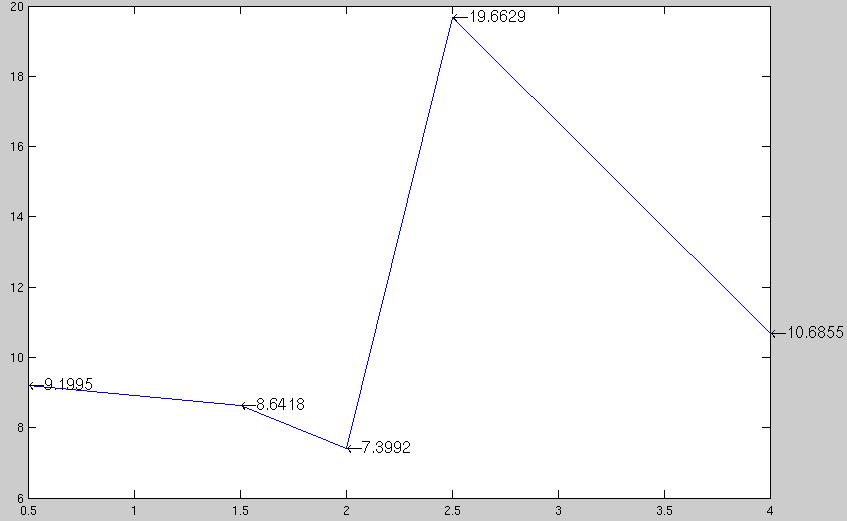
\includegraphics[scale=0.50]{Figures/rapport_tmu.png}
	\caption{$T(\mu)$}
	\label{figure:tmu}
\end{figure}
On souhaite calculer la période de la trajectoire ayant pour conditions initiales $\theta_0 = \frac{\pi}{2}$ et $\omega_0 = 0$, et pour paramètres $\lambda = 2$ et $\mu$ prenant successivement les valeurs suivantes: 0.5, 1.5, 2, 2.5 et 4. La période correspond à 2 fois la durée du parcours allant du point $(\theta_{min}, 0)$ à $(\theta_{max}, 0)$ étant donné la symétrie du problème.

\begin{flalign*}
	C &= \frac{1}{2} \dot{\theta}^2 + H(\theta)&\\
	\dot{\theta} = \frac{\mathd \theta}{\mathd t}&= \pm \sqrt{2(C - H(\theta))}&
\end{flalign*}

\begin{flalign*}
	T &= 2(t(\theta_{min}) - t(\theta_{max}))&\\
	  &= \int_{t(\theta_{min})}^{t(\theta_{max})}dt&\\
	  &=\sqrt{2} \int_{\theta_{min}}^{\theta_{max}} \frac{\mathd \theta}{\sqrt{C - H(\theta)}}&
\end{flalign*}

\underline{On calcule C aux conditions initiales}:
\begin{flalign*}
	C &= \frac{1}{2} \omega_0^2 + H(\theta_0)&\\
	  & = H(\theta_0)&\\
	  & = \cos{\theta_0} + \frac{1}{2}\frac{\lambda}{\mu}\left(
	  		\sqrt{\mu^2 + 1 -2\mu\cos{\theta_0}} - 1
	      \right)^2&\\
	  & =\frac{1}{2}\frac{\lambda}{\mu}\left(
	  		\sqrt{\mu^2 + 1} - 1
	      \right)^2&
\end{flalign*}

Avec $\lambda=2$:
\begin{flalign*}
	  C & =\frac{1}{\mu}\left(
	  		\sqrt{\mu^2 + 1} - 1
	      \right)^2&
\end{flalign*}

\underline{$H(\theta)$ pour $\lambda = 2$:}
\begin{flalign*}
	H(\theta) &= cos{\theta} + \frac{1}{\mu}\left(
					\sqrt{\mu^2 +1 -2\mu\cos{\theta}} - 1
	             \right)^2&
\end{flalign*}

\begin{leftbar}
\textbf{Exemple :} $\mu = 4$\\
On observe sur le portrait de phase (voir Annexe A) que la vitesse de la trajectoire s'annule aux points $\theta_{min} = -\frac{\pi}{2}$ et $\theta_{max} = \frac{\pi}{2}$.
\begin{flalign*}
	C &= \frac{1}{4}(\sqrt{17}-1)^2 \approx 2.4384&\\
	H(\theta) &= cos{\theta} + \frac{1}{4}(\sqrt{17-8\cos{\theta}}-1)^2&\\
	T &=\sqrt{2} \int_{\theta_{min}}^{\theta_{max}} \frac{\mathd \theta}{\sqrt{C - H(\theta)}} \approx 10.6855&
\end{flalign*}
\end{leftbar}

A l'aide de la figure \ref{figure:tmu}, on observe que les phénomènes pour $\mu=0.5, 1.5, 2, 4$ sont similaires, leur période est environ égale à 10. De plus on observe sur les portraits de phase (Annexe A) que les trajectoires de phase sont semblables. Le cas $\mu = 2.5$ est à part, on peut observer un changement de dynamique au niveau du portrait de phase, ce qui se traduit par une période doublée, et donc une vitesse de parcours divisée par deux.
\newpage

\paragraph{Matlab}\mbox{}\\
\begin{lstlisting}
function pr3001_B
    x_min=[pi/2 pi/2 1.3181-(pi/2 - 1.3181)+0.02 -pi/2 -pi/2];
    x_max=[3*pi/2  (1.8235-pi/2)+1.8235 pi/2-0.02 pi/2 pi/2];
    ...
    T=zeros(1,length(mu));
    for i=1:length(mu)
    	...
    	% période pour chaque mu (lambda fixé)
    	T(i) = quad(@periode, x_min(i), x_max(i),[],[], lambda, mu(i));
    end

    % affichage de la période en fonction de mu
    T = real(T);
    figure
    periodePlot(T, mu);
end

% Affiche la courbe représentant la période T (vecteur) en fonction de mu (vecteur).
function periodePlot(T, mu)
    plot(mu,T);
    title('T(mu)');

    for i=1:length(mu)
        str=strcat('\leftarrow ', num2str(T(i)));
        text(mu(i), T(i), str, 'FontSize', 14)
    end
end

function y=periode(x, lambda, mu)
    C= 0.5 * (lambda/mu) * (sqrt(mu^2 + 1) - 1)^2;
    y=sqrt(2)./sqrt(C - H_IntegPrem(lambda, mu, x));
end
\end{lstlisting}
Pour $\lambda=2$ et pour chaque $\mu$, on stocke le $\theta_{min}$ et le $\theta_{max}$ par lesquels la trajectoire de conditions initiales $(\theta_0=\frac{\pi}{2}, \omega_0=0)$ passe. Ces valeurs ont été relevées à l'aide des portraits de phase (voir Annexe A).\\

On calcule ensuite T pour chaque $\mu$ en intégrant la fonction \emph{periode} de $\theta_{min}$ jusqu'à $\theta_{max}$ à l'aide de $quad$. La courbe représentant $T(\mu)$ est finalement affichée grâce à la fonction \emph{periodePlot} (cf. figure \ref{figure:tmu}).
\newpage

\section{Cas avec frottement}
\subsection{Diagramme de bifurcation}
Comme indiqué dans le document \emph{Systèmes dynamiques et équations différentielles}, le diagramme de bifurcation est destiné à représenter la nature des points d'équilibre en fonction des paramètres du modèle. On souhaite dans notre cas représenter la nature des points d'équlibre en fonction de $\mu$, qui définit le point d'accroche du ressort, et de $\alpha$, le coefficient de frottement de l'anneau sur le cercle.

\begin{flalign*}
	&\ddot{\theta} + \alpha\dot{\theta} + h(2,\mu;\theta) = 0&\\
	&\ddot{\theta} + \alpha\dot{\theta} + sin{\theta} \left( -1 + \lambda - \frac{\lambda}{\sqrt{\mu^2 + 1 -2\mu\cos{\theta}}} \right) = 0&
\end{flalign*}

\underline{Système différentiel autonome de dimension 2}:
\begin{flalign*}
	&\begin{cases}
		\dot{x_1}(t) = f_1(x_1(t), x_2(t))\\
		\dot{x_2}(t) = f_2(x_1(t), x_2(t))
	\end{cases}&
\end{flalign*}
$F = (f_1(t), f_2(t))$\\

On pose :
\begin{flalign*}
	&\begin{cases}
		x_1 = \theta\\
		x_2 = \dot{\theta}
	\end{cases}&
\end{flalign*}

D'où (avec $\lambda=2$) :
\begin{flalign*}
	&\begin{cases}
		\dot{x_1} = \dot{\theta} = x_2\\
		\dot{x_2} = \ddot{\theta} = -\alpha x_2 - \sin{x_1} \left( 1 - \frac{2}{\sqrt{\mu^2 + 1 -2\mu\cos{x_1}}} \right)
	\end{cases}&
\end{flalign*}

\underline{Points d'équilibre}:\\
Les points d'équilibres dans le cas avec frottement peuvent être étudiés à partir de l'équation différentielle (ou à partir du système autonome de dimension 2) :
\begin{flalign*}
	&\ddot{\theta} + \alpha\dot{\theta} + sin{\theta} \left( -1 + \lambda - \frac{\lambda}{\sqrt{\mu^2 + 1 -2\mu\cos{\theta}}} \right) = 0&
\end{flalign*}

On fixe $\ddot{\theta} = 0$ et $\dot{\theta} = 0$ dans l'équation différentielle, les valeurs des points d'équilibre sont obtenues en résolvant l'équation :
\begin{flalign*}
	&\sin{\theta} \left( -1 + \lambda - \frac{\lambda}{\sqrt{\mu^2 + 1 -2\mu\cos{\theta}}} \right) = 0&
\end{flalign*}
Cette équation est la même que celle obtenue dans le cas sans frottement, les points d'équilibres sont donc indépendants du frottement.
On retrouve donc les points d'équilibre précédents :\\
$\theta^*=0$ et $\theta^* = \pi \quad$ ($\theta^* = k\pi, \quad k \in \mathbb{Z}$)\\
\begin{flalign*}
\theta^* &= \pm \cos^{-1}{\left( \frac{\left(\frac{\lambda}{\lambda-1}\right)^2 -\mu^2 -1}{-2\mu} \right)}&\\
         &= \pm \cos^{-1}{\left( \frac{\mu^2 - 3}{2\mu} \right)}, \quad \lambda=2&
\end{flalign*}

Ces solutions peuvent être représentées graphiquement de la manière suivante, avec en bleu les points d'équilibre stables et en rouge les points d'équilibre instables :
\begin{figure}[h!]
	\centering
	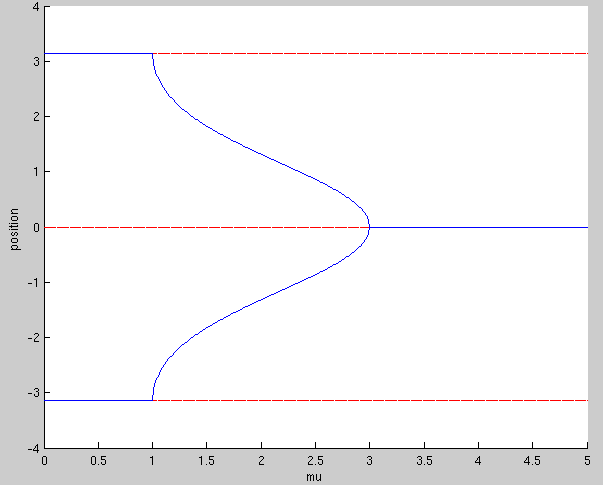
\includegraphics[scale=0.59]{Figures/rapport_bifur1.png}
	\caption{Représentation des points d''équilibre en fonction de $\mu$ ($\lambda=2$)}
\end{figure}
\newpage

\underline{Système non-linéaire}:\\
Nous sommes dans le cas d'un système non-linéaire, nous cherchons donc à étudier son comportement au voisinage des points d'équilibre.\\

Soit $x^* = (x_1^*,x_2^*)$, 1 point d'équilibre du système, on souhaite calculer la matrice jacobienne de $f_i $ au voisinage de $x^*$.
\begin{flalign*}
	\frac{\partial f_1}{\partial x_1} &= 0&\\
	\frac{\partial f_1}{\partial x_2} &= 1&\\
	\frac{\partial f_2}{\partial x_1} &= -\frac{\partial}{\partial x_1} \left( \sin{x_1}\left( 1 - \frac{2}{\sqrt{\mu^2 +1 -2\mu\cos{x_1}}} \right) \right)&\\
	&= -\cos{x_1}\left( 1 - \frac{2}{\sqrt{\mu^2 +1 -2\mu\cos{x_1}}} \right) -2\mu\frac{\sin^2{x_1}}{(\mu^2 +1 -2\mu\cos{x_1})^{3/2}}&\\
	\frac{\partial f_2}{\partial x_2} &= -\alpha&\\
	A(x^*) &= \left[
		\begin{matrix}
		  0 & 1 \\
		  \frac{\partial f_2}{\partial x_1} & -\alpha
		\end{matrix}
 	\right]&
\end{flalign*}

On a :
\begin{flalign*}
	&\begin{cases}
		Tr(A) = -\alpha\\
		Det(A) = -\frac{\partial f_2}{\partial x_2}\\
		\Delta(A) = tr(A)^2 - 4*det(A)
	\end{cases}&
\end{flalign*}

On souhaite représenter le système au voisinage d'un point d'équilibre $x^*$ stable, et donc délimiter les zones de \textbf{noeud attractif}, de \textbf{spirale attractif} et de \textbf{centre}.\\

En rassemblant les conditions de ces trois zones, on obtient les conditions suivantes :
\begin{flalign*}
	&\begin{cases}
		Det(A) \geq 0\\
		Tr(A) \leq 0
	\end{cases}&
\end{flalign*}
Or, $Tr(A) = -\alpha$ et $\alpha \geq 0$, une des deux conditions est toujours remplie. Il faut donc ensuite choisir $x^*$ tel que $-\frac{\partial f_2}{\partial x_2} \geq 0$ afin que $Det(A) \geq 0$. Le point d'équilibre ainsi choisi sera stable.
\newpage

\begin{figure}[h!]
	\centering
	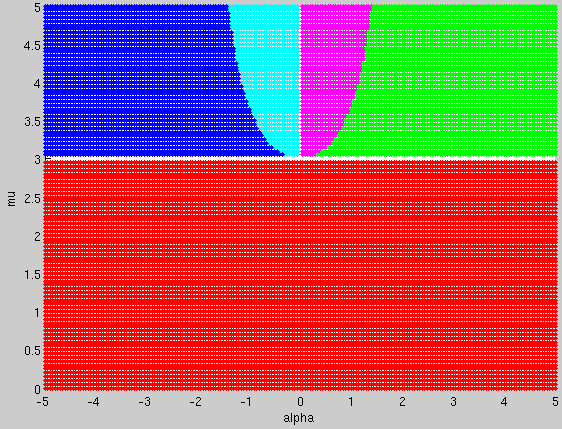
\includegraphics[scale=0.59]{Figures/rapport_bifur2.png}
	\caption{Diagramme de bifurcation}
\end{figure}

Le diagramme ci-dessus montre :
\begin{itemize}
	\item Pour $\alpha = 0$, il n'y a pas de frottements, on se ramène au cas de la partie B. Les points d'équilibre stables sont de type centré.
	\item Pour un $\mu$ donné et $\alpha$ dans la zone à gauche du trait bleu, les points d'équilibre sont de type spirale attractif. Le système s'amortit avec des oscillations.
	\item Pour un $\mu$ donné et $\alpha$ dans la zone à droite du trait bleu, les points d'équilibre sont de type noeuf attractif. Le mouvement du système est très amorti, sans oscillations.
\end{itemize}

\begin{leftbar}
	\textbf{N.B.} Les points d'équilibre instables sont relevés pour un $Det(A) < 0$ et ont pour nature le point selle. Les points instables ne sont pas représentés sur le diagramme ci-dessus.
\end{leftbar}
\newpage

\paragraph{Matlab}\mbox{}\\
\begin{lstlisting}
% Diagramme de bifurcation
function plotBifurcation(mu)
    lambda = 2;
    alphaFricArray = zeros(1, length(mu));

    for i=1:length(mu)
        mu(i)
        ptEqui = [0 pi];

        % points d'équilibre du système
        if (mu(i) < (lambda/(lambda-1)) + 1) && (mu(i) > (lambda/(lambda-1)) - 1) % 4 points
            ptEqui(end + 1) = equiArccos(lambda, mu(i));
        end

        % on choisit un point d'équilibre tel que le système soit stable (det(A) > 0
        % sachant que tr(A) < 0)
        for j=1:length(ptEqui)
            detPtEqui = det(ptEqui(j), mu(i))
            if detPtEqui >= 0
                ptEquiChoisi = ptEqui(j);
                break;
            end
        end

        alphaFricArray(i) = alphaFriction(ptEquiChoisi, mu(i));
    end

    plot(alphaFricArray, mu);
    title('Diagramme de bifurcation')
    xlabel('alpha')
    ylabel('mu')
end

% Calcule le déterminant de la matrice jacobienne pour lambda=2 et en
% fonction de lambda et x1 (theta).
function y=det(x1, mu)
    y = cos(x1)*(1 - (2/sqrt(mu^2 + 1 -2*mu*cos(x1)))) ...
        + 2*mu*((sin(x1)^2)/((mu^2 + 1 -2*mu*cos(x1))^(3/2)));
end

% Calcule alpha en fonction de x1 et mu
function y=alphaFriction(x1, mu)
    y = 2*sqrt(det(x1,mu));
end
\end{lstlisting}

La fonction \emph{plotBifurcation} effectue les étapes suivantes :
\begin{enumerate}
	\item fixe $\lambda$
	\item pour chaque $\mu$ :
	\begin{enumerate}
		\item calcule det(A) pour chaque point d'équilibre du système
		\item choisi le premier point d'équilibre pour lequel $det(A) \geq 0$ (stabilité)
		\item calcule $\alpha$ en fonction de $\mu$ et du point d'équilibre choisi
	\end{enumerate}
	\item trace $\mu(\alpha)$ (diagramme de bifurcation)

\end{enumerate}
\newpage

\subsection{Stabilisation en un point}
Nous avons établi précédemment le système différentiel autonome de dimension 2 suivant :
\begin{flalign*}
	&\begin{cases}
		\dot{x_1}(t) = f_1(x_1(t), x_2(t))\\
		\dot{x_2}(t) = f_2(x_1(t), x_2(t))
	\end{cases}&
\end{flalign*}

A partir de ce système et à l'aide de Matlab nous pouvons simuler divers cas et racer la trajectoire correspondante pour $\theta_0$ et $\mu$ fixés, ainsi qu'un intervalle de temps, un amortissement $\alpha$, et un $\omega_0$ donnés.\\

Nous pouvons par exemple observer ci-dessous une réprésentation de spirale attractif pour $\theta_0=0, \mu=2, \alpha=0.2,\omega_0=2$. Dans ce cas, le système se stabilise en $\theta \simeq 7.7 rad$.

\begin{figure}[h!]
	\centering
	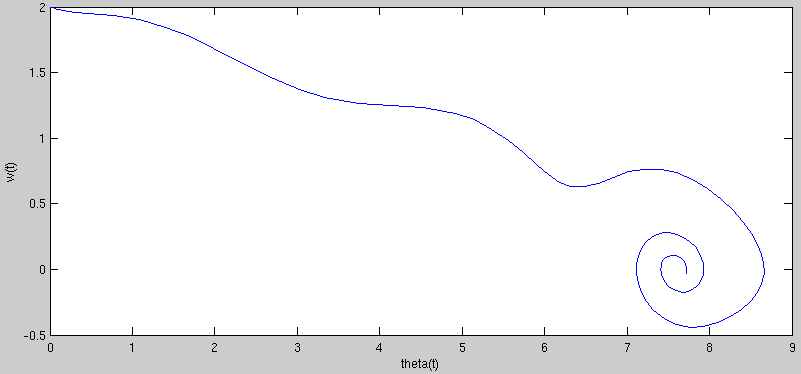
\includegraphics[scale=0.59]{Figures/rapport_traj_spiral.png}
	\caption{spirale attractif pour $\theta_0=0, \mu=2, \alpha=0.2,\omega_0=2$}
\end{figure}

\begin{figure}[h!]
	\centering
	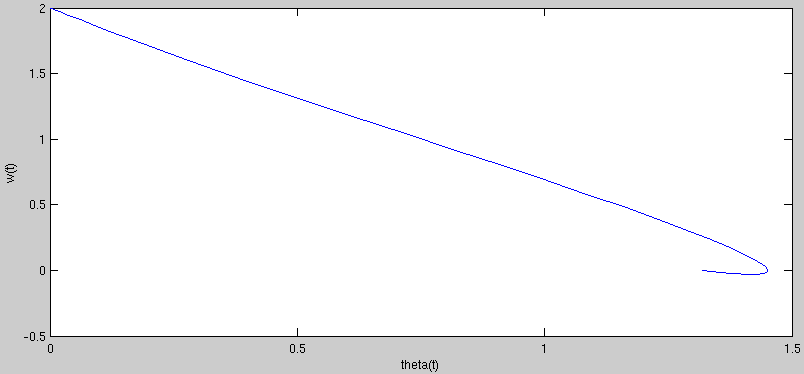
\includegraphics[scale=0.59]{Figures/rapport_traj_noeud.png}
	\caption{noeud attractif pour $\theta_0=0, \mu=2, \alpha=1.5,\omega_0=2$}
\end{figure}

\begin{figure}[h!]
	\centering
	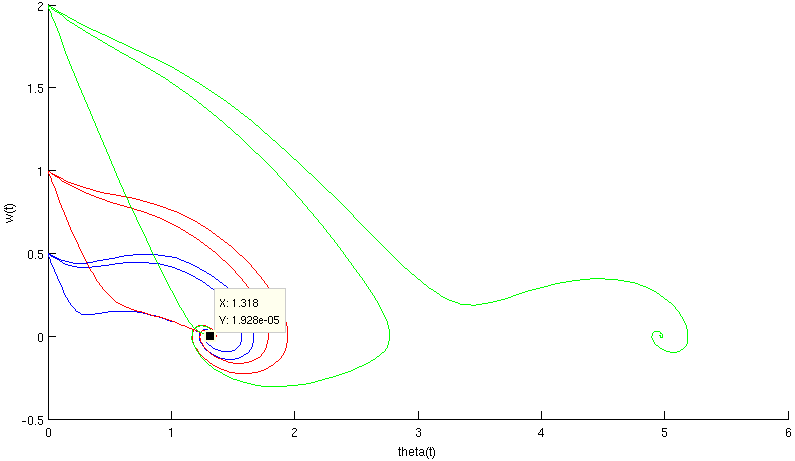
\includegraphics[scale=0.6]{Figures/rapport_stab.png}
	\caption{trajectoires pour $\omega_0=0.5$ (bleu), $\omega_0=1$ (rouge), $\omega_0=2$ (vert) et pour $\alpha=$[0.5 0.6 2]}
	\label{fig:stab}
\end{figure}

On peut observer sur la figure \ref{fig:stab} plusieurs trajectoires pour des $\omega_0$ et des $\alpha$ différents. Chaque couleur correspond à une valeur de $\omega_0$. On peut ainsi voir que pour un $\alpha \geq 0.6$, toutes les trajectoires convergent en $(\theta \simeq 1.31, \omega = 0)$ ce qui correspond à un point d'équilibre stable pour le système avec $\lambda=2, \mu=2$. Pour $\alpha < 0.6$, on commence à voir apparaître des trajectoires qui se stabilisent en un autre point. Notamment pour $\alpha=0.5$ et $\omega_0 = 2$, on voit que la trajectoire se stabilise en $4.96 rad$.

\newpage

\paragraph{Matlab}\mbox{}\\
\begin{lstlisting}
function pr3001_B
	...
    % Représentation spirale attractif
    figure('name', 'spirale attractif')
    reptraj([0;2],30,0.2,2)

    % Représentation noeud attractif
    figure('name', 'noeud attractif')
    reptraj([0;2],30,1.5,2)

    % Trajectoires pour divers alpha et omega0
    figure
    colors=['b', 'r', 'g'];
    w=[0.5 1 2];
    a=[0.5 0.6 2];
    hold on
        for i=1:length(a)
            for j=1:length(w)
                reptraj([0;w(j)],30,a(i),2,0, colors(j))
            end
        end
    hold off
end

% Representation d'une trajectoire
% reptraj([x0;w0], temps final, amortissement, mu)
% bleu -> x(t) ; vert -> v(t)
function reptraj(x0,tf,a,mu)
    [t,x]=ode45(@syst,[0 tf],x0,[],a,mu);

    subplot(2,1,1)
    plot(t,x)
    title(['Parametres: \alpha=' num2str(a) '   mu=' num2str(mu) '  ;'...
        '  Conditions initiales: \theta_0=' num2str(x0(1)) '  \omega_0=' num2str(x0(2)) ])
    xlabel('t')
    grid
    axis([0 30 -10 10])

    subplot(2,1,2)
    plot(x(:,1),x(:,2))
    xlabel('theta(t)')
    ylabel('w(t)')
end

% Système différentiel autonome de dimension 2
function dxdt=syst(~,x,a,mu)
	dxdt=[x(2);-a*x(2)-sin(x(1))*(1 - (2/sqrt(mu^2 + 1 -2*mu*cos(x(1)))))];
end
\end{lstlisting}

\newpage

\appendix
\section{Annexe: portraits de phase}
\begin{figure}[h!]
	\centering
	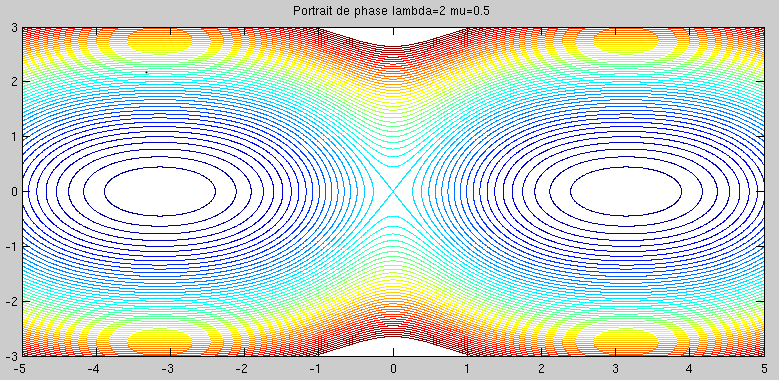
\includegraphics[scale=0.64]{Figures/rapport_pp05.png}
\end{figure}

\begin{figure}[h!]
	\centering
	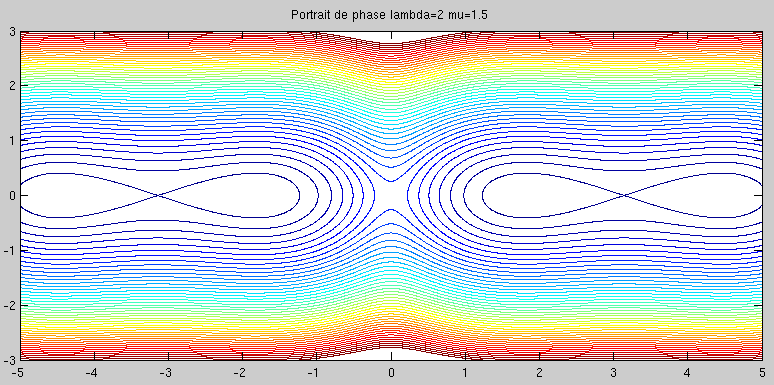
\includegraphics[scale=0.65]{Figures/rapport_pp15.png}
\end{figure}

\begin{figure}[h!]
	\centering
	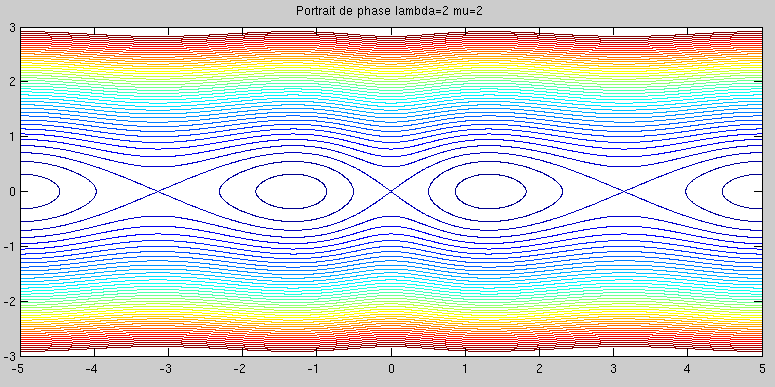
\includegraphics[scale=0.65]{Figures/rapport_pp20.png}
\end{figure}
\newpage % fix
\begin{figure}[h!]
	\centering
	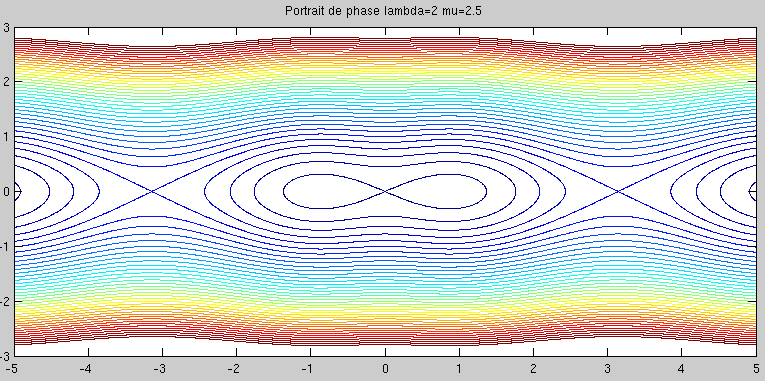
\includegraphics[scale=0.66]{Figures/rapport_pp25.png}
\end{figure}
\newpage
\begin{figure}[h!]
	\centering
	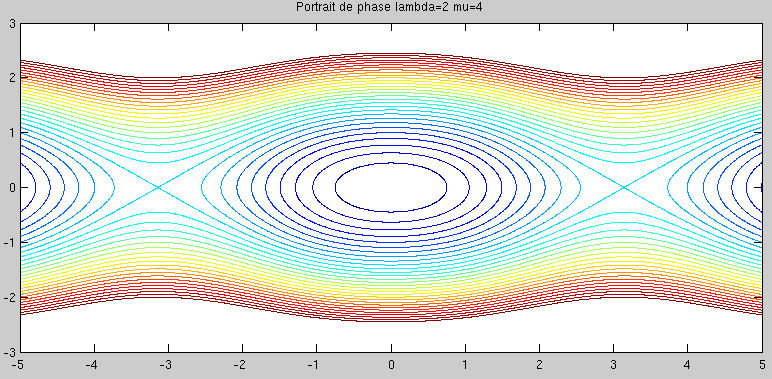
\includegraphics[scale=0.65]{Figures/rapport_pp40.png}
\end{figure}


\newpage
\section{Annexe: Code complet}
\lstinputlisting{../pr3001_B.m}

\end{document}
